\documentclass[12pt]{article}

\usepackage[utf8]{inputenc}
\usepackage[german]{babel}
\usepackage{graphicx}
\usepackage{subfiles}
\usepackage{caption,subcaption} % Subfigures
\usepackage{fancyhdr} % Header/Footer
\usepackage{pgfplots}

\graphicspath{ {./assets/images/} }

% Sans-serif
\renewcommand{\familydefault}{\sfdefault}

% Header
\pagestyle{fancy}
\renewcommand{\headrulewidth}{0pt}
\fancyhf{}
\lhead{P-Seminar KUNO}
\chead{Digitale Spiele (12-17)}
\rhead{Noah Jutz}
\cfoot{\thepage}

\title{
    KUNO - Kind-Eltern-Kinderklinik: Digitale Spiele für 12 bis 17-jährige Patienten
    \newline\vspace{0.5cm}
    \centering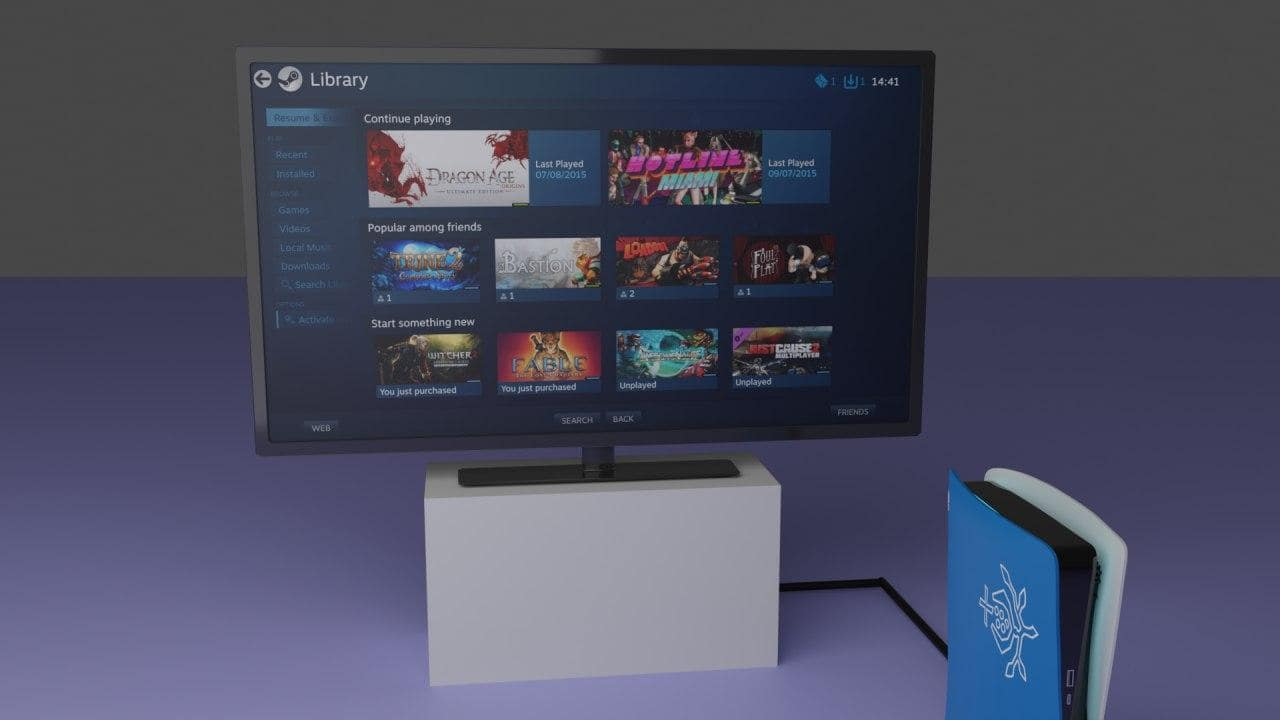
\includegraphics[width=\textwidth]{ps5_steam.jpg}
}
\author{Noah Jutz}
\date{}

\begin{document}
    \maketitle

    \newpage
    \tableofcontents

    \newpage
    \section{Berufs- und Studienorientierung}
    \subsection{Studium und Kosten}
    \subfile{sections/bus/studium_kosten.tex}

    \newpage
    \subsection{Berufsbewerbung und Lebenslauf}
    \subfile{sections/bus/bewerbung_lebenslauf.tex}

    \subsection{Praktikumsnachweise}
    \subfile{sections/bus/praktikumsnachweise.tex}

    \subsection{Selbsteinschätzung}
    \subfile{sections/bus/selbsteinschaetzung.tex}

    \newpage
    \subsection{Berufsinfos}
    \subfile{sections/bus/berufsinfos.tex}

    \newpage
    \subsection{Qualifikationen}
    \subfile{sections/bus/qualifikationen.tex}

    \newpage
    \section{Projekt}
    \subsection{Intention}
    \subfile{sections/projekt/intention.tex}

    \newpage
    \subsection{Vision}
    \subfile{sections/projekt/vision.tex}

    \newpage
    \subsection{Bericht}
    \subfile{sections/projekt/bericht.tex}

    \newpage
    \subsection{Reflexion}
    \subfile{sections/projekt/reflexion.tex}

    \newpage
    \subsection{Fragenkatalog}
    \subfile{sections/projekt/fragenkatalog.tex}

    \newpage
    \subsection{Auswertung}
    \subfile{sections/projekt/auswertung.tex}

    \newpage
    \subsection{Visualisierung}
    \subfile{sections/projekt/visualisierung.tex}

    \newpage
    \subsection{Resumé}
    \subfile{sections/projekt/resume.tex}
\end{document}
